% !TEX encoding = UTF-8 Unicode
% !TEX TS-program = XeLaTeX
\documentclass[UTF8,12pt,letterpaper,oneside]{amsart}
\usepackage[letterpaper]{geometry}
\geometry{top=1.0in, bottom=1.0in, left=1.0in, right=1.0in}
\usepackage{setspace}
%\doublespacing
\usepackage{hyperref}
%\usepackage{times}
\usepackage{graphicx}
\usepackage{rotating}
\usepackage{multirow}
\usepackage{lineno} 
\usepackage{fancyhdr}
\usepackage{hanging}
\usepackage{listings}
\pagestyle{fancy}
\rhead{\textsc{La \& Yang} \thepage} 
\renewcommand{\headrulewidth}{0pt} 
\renewcommand{\footrulewidth}{0pt} 
\setlength\headsep{0.333in}
\usepackage{tikz}
\usetikzlibrary{arrows,automata}
\begin{document}

\noindent Minh \textsc{La}, Luke \textsc{Yang}\\
EE 201\\
Instructor Gandhi \textsc{Puvvada}\\
Due Dec $3$rd\\
Final Project Report


\section{Summery}

This final project report is on a TicTacToe game implemented on Nexys3 FPGA Board with a VGA display. It consists of a core machine that handles the gaming, and a front-end that coordinates the I/O signal, calculates all graphical content, and calls the \texttt{hvsync\_generator} module to produce the display. 

\section{Backend}


\begin{tikzpicture}[shorten >=1pt,node distance=4cm,auto,initial text={\texttt{Reset}}]

\node[state,initial]  (INIT)                         {\texttt{initial}};
\node[state]          (CLEAR) [right of=INIT]        {\texttt{clear}};
\node[state]          (CHECK) [right of=CLEAR]       {\texttt{check}};
\node[state,accepting](P1WIN) [above of=INIT] {\texttt{p1win}};
\node[state,accepting](P2WIN) [below right of=CLEAR] {\texttt{p2win}};
\node[state,accepting](DRAW)  [above right of=CHECK]       {\texttt{draw}};



\path[->] (INIT)  edge node {\texttt{Start}} (CLEAR)
          (CLEAR) edge node {\texttt{1}}     (CHECK)
          (CHECK) edge [bend right=30]node {all p1win conditions} (P1WIN)
                  edge [bend left=30] node {all p2win conditions} (P2WIN)
                  edge [bend right=40]node {draw condition} (DRAW)
          (P1WIN) edge [bend right=20] node {\texttt{Start}} (CLEAR)           
          (P2WIN) edge [bend left=20] node {\texttt{Start}} (CLEAR)
          (DRAW)  edge [bend right]node {\texttt{Start}} (CLEAR);
\end{tikzpicture}


As shown in the diagram, we implemented a six-state state machine in the core design, with initial state being \texttt{initial} upon an asynchronous \texttt{Reset} signal from \texttt{Button\_Up}. Push button \texttt{Button\_Down} produces signal \texttt{Start}, which brings the system into \texttt{clear} state. Inside \texttt{clear} state, the system initializes all the local registers for game bookkeeping. These registers include \texttt{gameOver} true when a winner has been found, \texttt{location[3:0]} keeping track of the cursor, \texttt{p1Win} true when player $1$ wins, \texttt{p2Win} true when player $2$ wins, \texttt{draw} true when the board full but no one wins, and \texttt{[1:0]mapBoard[8:0]} recording all moves on board in an array. After initialization, the system moves into \texttt{check} unconditionally.

In \texttt{check} state, two players play in turns and the system processes input signals. The player can move the cursor around the board using \texttt{Button\_Left} and \texttt{Button\_Right}, and the value of \texttt{location} changes accordingly. After placing the cursor at a desired location, the player can confirm the selection by pressing \texttt{Button\_Center}, which generates \texttt{Enter} signal. Upon this signal, the system in \text{check} state first updates \texttt{mapBoard[location]}, where \texttt{location} represents the cursor's location. The value of \texttt{mapBoard[location]} is updated to $1$ for player one, and $2$ for player two. Players take turn to play this game manually, as signal \texttt{player} is toggled by \texttt{Switch0}. After updating \texttt{mapBoard} array, the system goes through each row, each column, and each diagonal, and checks if the values are the same. If they are the same, the \texttt{gameOver} flag is set on, and the system moves into accepting states \texttt{p1win} or \texttt{p2win}, depending on whether it finds \texttt{1, 1, 1} or \texttt{2, 2, 2}. At the end of each round's check, the system also detects whether the board has been full. If the board has been full but \texttt{gameOver} flag has not been set on, the system moves into \texttt{draw} state since no further moves can be taken and neither player has won. If none of the aforementioned jump conditions are satisfied, the system stays in \texttt{check} state and waits for next input. The three accepting states \texttt{p1win}, \texttt{p2win}, and \texttt{draw} simply update the bookkeeping registers, and wait for \texttt{Start} signal to bring the system back to \texttt{clear}.

\section{Front End}

The front-end is the top design of this project, and it calls the backend and \texttt{hvsync\_generator} as two subroutines. After this, it starts its own state machine.


\begin{tikzpicture}[shorten >=1pt,node distance=4.5cm,auto,initial text={\texttt{Reset}}]


\node[state,initial,accepting]  (G00)                {\texttt{grid[0][0]}};
\node[state,accepting]          (G10) [right of=G00] {\texttt{grid[1][0]}};
\node[state,accepting]          (G20) [right of=G10] {\texttt{grid[2][0]}};
\node[state,accepting]          (G01) [below of=G00] {\texttt{grid[0][1]}};
\node[state,accepting]          (G11) [right of=G01] {\texttt{grid[1][1]}};
\node[state,accepting]          (G21) [right of=G11] {\texttt{grid[2][1]}};
\node[state,accepting]          (G02) [below of=G01] {\texttt{grid[0][2]}};
\node[state,accepting]          (G12) [right of=G02] {\texttt{grid[1][2]}};
\node[state,accepting]          (G22) [right of=G12] {\texttt{grid[2][2]}};

\path[->] (G00)  edge [bend right=20]  node {\texttt{Right}}  (G10)
                 edge [bend left=25]  node {\texttt{Left}}  (G22)
          (G10)  edge [bend right=20]  node {\texttt{Left}}   (G00)
                 edge [bend right=20]  node {\texttt{Right}}  (G20)
          (G20)  edge [bend right=20]  node {\texttt{Left}}   (G10)
                 edge [bend left=5]  node {\texttt{Right}}  (G01)
          (G01)  edge [bend left=5]  node {\texttt{Left}}  (G20)
                 edge [bend right=20]  node {\texttt{Right}}  (G11)
          (G11)  edge [bend right=20]  node {\texttt{Left}}   (G01)
                 edge [bend right=20]  node {\texttt{Right}}  (G21)
          (G21)  edge [bend right=20]  node {\texttt{Left}}   (G11)
                 edge [bend left=5]  node {\texttt{Right}}  (G02)
          (G02)  edge [bend left=5]  node {\texttt{Left}}  (G21)
                 edge [bend right=20]  node {\texttt{Right}}  (G12)
          (G12)  edge [bend right=20]  node {\texttt{Left}}   (G02)
                 edge [bend right=20]  node {\texttt{Right}}  (G22)
          (G22)  edge [bend right=20]  node {\texttt{Left}}   (G12)
                 edge [bend left=25]  node {\texttt{Right}}  (G00);

\end{tikzpicture}



This nine-state state machine corresponds to the $3 \times 3$ grid in the graphical front-end, and it shares the same set of control signals \texttt{Reset}, \texttt{Start}, \texttt{Left}, \texttt{Right}, and \texttt{Enter}. To ensure proper synchronization with the backend, it also reads values of \texttt{p1Win}, \texttt{p2Win}, \texttt{draw}, and \texttt{player} from the backend. The nine states represents the nine grids in the game as well as the nine-element \texttt{mapBoard[]} array in the backend. The system can jump back and forth among the nine states using \texttt{Left} and \texttt{Right} since the states are circular doubly-linked. Upon \texttt{Reset}, the system resets all local registers for colored area enabling, and goes into \texttt{G00} state. In fact, the system also waits for the core to get into \texttt{check} state, represented by \texttt{p1Win\ ||\ p2Win\ ||\ draw} being false. When the game is in session, the system updates the cursor location based on current state, and reacts to \texttt{Enter}, \texttt{Left}, and \texttt{Right} signals. Signal \texttt{Enter} enables green or blue color being displayed at current cursor location depending on \texttt{player} value. Signals \texttt{Left} and \texttt{Right} simply moves the state back and forth, with the effect of cursor moving.

we have also used seven-segment-display LEDs to display the game's status. The first display \texttt{SSD0} displays the player's number ($0$ or $1$). The next three displays \texttt{SSD1}, \texttt{SSD2}, and \texttt{SSD3} correspond to game's results: \texttt{draw}, \texttt{p2Win}, and \texttt{p1Win}.





\end{document}

